
\documentclass[11pt]{article}
\usepackage[margin=0.8in]{geometry}
\usepackage{amsmath,amssymb,booktabs,array,longtable}
\usepackage{hyperref}
\usepackage{enumitem}
\usepackage{graphicx}
\usepackage{float}
\usepackage{caption}
\setlist{nosep}

\begin{document}

\begin{center}
{\Large\textbf{Shiv Nadar University Chennai}}\\
\textbf{CS3807 -- Deep Learning Laboratory}\\
\textbf{Experiment 2}\\
{\large\textbf{Implementation of a Multi-Layer Perceptron (MLP) for Multi-Class Image Classification}}
\end{center}

\renewcommand{\arraystretch}{1.25}

\begin{tabular}{|p{3.8cm}|p{8cm}|p{2cm}|}
\hline
Degree \& Branch & B.Tech Artificial Intelligence \& Data Science & Semester V\\ \hline
Subject Code \& Name & CS3807 -- Deep Learning Laboratory & AY: 2026--27\\ \hline
\end{tabular}

\section*{1. Objective}
Implement an MLP using TensorFlow/Keras on the Fashion-MNIST dataset. Learn image preprocessing, flattening, model construction, training, evaluation, and automated hyperparameter optimization.

\section*{2. Learning Outcomes}
Students will be able to:
\begin{enumerate}
\item Explain the architecture of an MLP.
\item Preprocess image datasets.
\item Build and train an MLP.
\item Evaluate classification performance.
\item Perform automated hyperparameter optimization.
\item Recommend the best model configuration.
\end{enumerate}

\section*{3. Background Theory}
An MLP consists of an input layer, hidden layers and an output layer.

\[
z^{(l)}=W^{(l)}a^{(l-1)}+b^{(l)},\qquad
a^{(l)}=f(z^{(l)})
\]

Output layer:
\[
\hat y=\mathrm{Softmax}(z)
\]

Loss:
\[
L=-\sum_i y_i\log(\hat y_i)
\]

Recommended architecture:

\begin{center}
784 $\rightarrow$ Dense(128, ReLU) $\rightarrow$ Dense(64, ReLU) $\rightarrow$ Dense(10, Softmax)
\end{center}

\section*{4. Dataset}
Dataset: Fashion-MNIST

Training Images: 60,000 \\
Testing Images: 10,000 \\
Classes: 10 \\
Image Size: $28\times28$

\section*{5. Image Preprocessing}

Fashion-MNIST images are stored as $28\times28$ matrices. Dense layers require a one-dimensional feature vector.

\[
28\times28=784
\]

Example:

\[
\begin{bmatrix}
10&20\\30&40
\end{bmatrix}
\rightarrow
[10,20,30,40]
\]

Perform the following preprocessing:

\begin{enumerate}
\item Load Fashion-MNIST.
\item Display sample images.
\item Flatten images.
\item Normalize pixels to [0,1].
\item Convert labels into one-hot vectors.
\end{enumerate}

\section*{6. Experimental Procedure}

\textbf{Task 1: Dataset Exploration}
\begin{itemize}
\item Load Fashion-MNIST.
\item Print dataset dimensions.
\item Display ten sample images.
\item Plot class distribution.
\end{itemize}

\textbf{Expected Output:}
Dataset summary and sample images.

\bigskip

\textbf{Task 2: Data Preprocessing}

\begin{itemize}
\item Flatten images.
\item Normalize pixel values.
\item Print tensor shapes before and after preprocessing.
\end{itemize}

\bigskip

\textbf{Task 3: Model Construction}

Construct an MLP with

\begin{itemize}
\item Input layer (784)
\item Dense(128, ReLU)
\item Dense(64, ReLU)
\item Dense(10, Softmax)
\end{itemize}

Display \texttt{model.summary()}.

\bigskip

\textbf{Task 4: Model Training}

Compile using

\begin{itemize}
\item Optimizer: Adam
\item Loss: Categorical Cross Entropy
\item Metric: Accuracy
\end{itemize}

Train for 20 epochs with batch size 32.

\bigskip

\textbf{Task 5: Model Evaluation}

Compute

\begin{itemize}
\item Accuracy
\item Precision
\item Recall
\item F1-score
\item Confusion Matrix
\item Classification Report
\end{itemize}
\section*{7. Source Code Repository}

The complete implementation of this experiment, including dataset exploration, data preprocessing, baseline MLP construction, model training, performance evaluation, hyperparameter optimization using RandomizedSearchCV,  has been made available through the following GitHub repository.

\bigskip

\noindent
\textbf{GitHub Repository:}

\url{https://github.com/Siddharth-G06/Deep-Learning-Lab/tree/main/Lab%202%20-%20Multi-Layer%20Perceptron}

\bigskip

The repository enables reproducibility of the experiment and allows the implementation to be executed, verified, and extended using the same methodology described in this report.

\section*{8. Hyperparameter Optimization}

Instead of manually selecting hyperparameters, students shall perform automated hyperparameter optimization using either \textbf{GridSearchCV} or \textbf{RandomizedSearchCV} (recommended) together with the SciKeras wrapper.

Optimize the following search space.

\begin{center}
\begin{tabular}{|p{5cm}|p{7cm}|}
\hline
Hyperparameter & Candidate Values\\
\hline
Hidden Layers & 1, 2, 3\\
Hidden Neurons & 32, 64, 128, 256\\
Learning Rate & 0.1, 0.01, 0.001\\
Batch Size & 16, 32, 64, 128\\
Epochs & 10, 20, 30\\
Optimizer & SGD, Adam, RMSProp\\
Activation Function & ReLU, Tanh, Sigmoid\\
Dropout Rate (Optional) & 0.0, 0.2, 0.5\\
\hline
\end{tabular}
\end{center}

\subsection*{Tasks}

\begin{enumerate}
\item Build a baseline MLP model.
\item Define the hyperparameter search space.
\item Perform Grid Search or Randomized Search using 5-fold cross-validation.
\item Record the best hyperparameter combination.
\item Retrain the model using the optimized hyperparameters.
\item Evaluate the optimized model on the testing dataset.
\item Compare the optimized model with the baseline model.
\end{enumerate}

\section*{9. Plots with Inference}

Generate the following plots.

\begin{enumerate}
\item Sample Images
\item Class Distribution
\item Training Accuracy vs Epoch
\item Validation Accuracy vs Epoch
\item Training Loss vs Epoch
\item Validation Loss vs Epoch
\item Confusion Matrix
\item Hyperparameter Search Results
\item Best Model Accuracy Comparison
\end{enumerate}

Write a 2--3 line inference for each plot.
\begin{figure}[H]
\centering
\includegraphics[width=0.8\linewidth]{Sample_Images.eps}
\caption{Sample Images from the Fashion-MNIST Dataset}
\end{figure}

\textbf{Inference:}

The sample images demonstrate the diversity of clothing categories available in the Fashion-MNIST dataset. Each grayscale image belongs to one of the ten predefined classes and serves as the input for the multi-class classification model.

\begin{figure}[H]
\centering
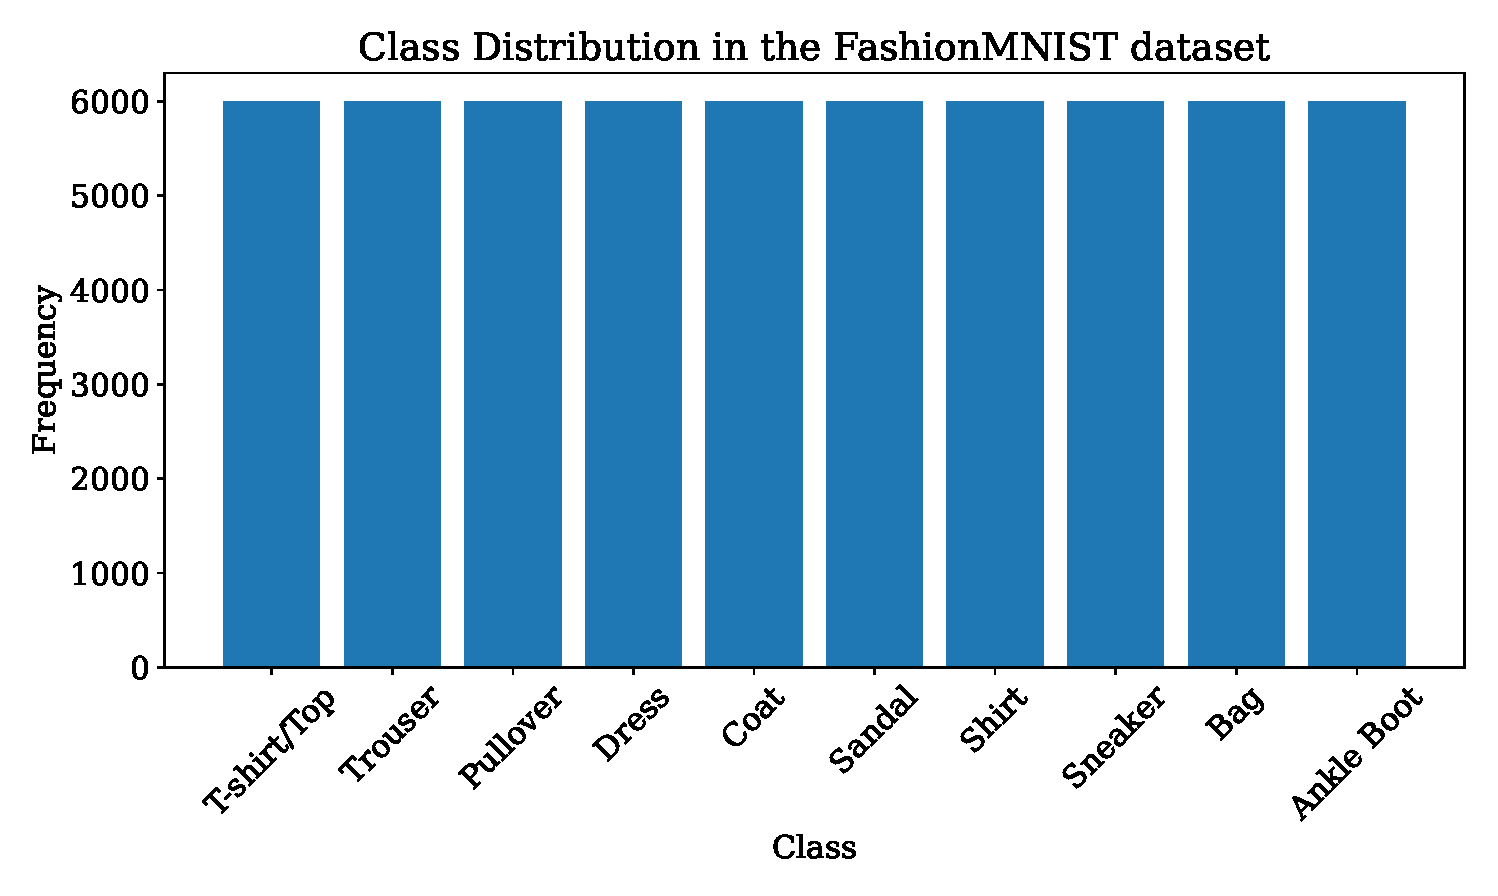
\includegraphics[width=0.75\linewidth]{Class_Distribution.eps}
\caption{Class Distribution of the Fashion-MNIST Dataset}
\end{figure}

\textbf{Inference:}

The class distribution is uniform, with approximately 6,000 training images in each category. This balanced dataset minimizes class imbalance and allows the MLP to learn each category without bias.

\begin{figure}[H]
\centering
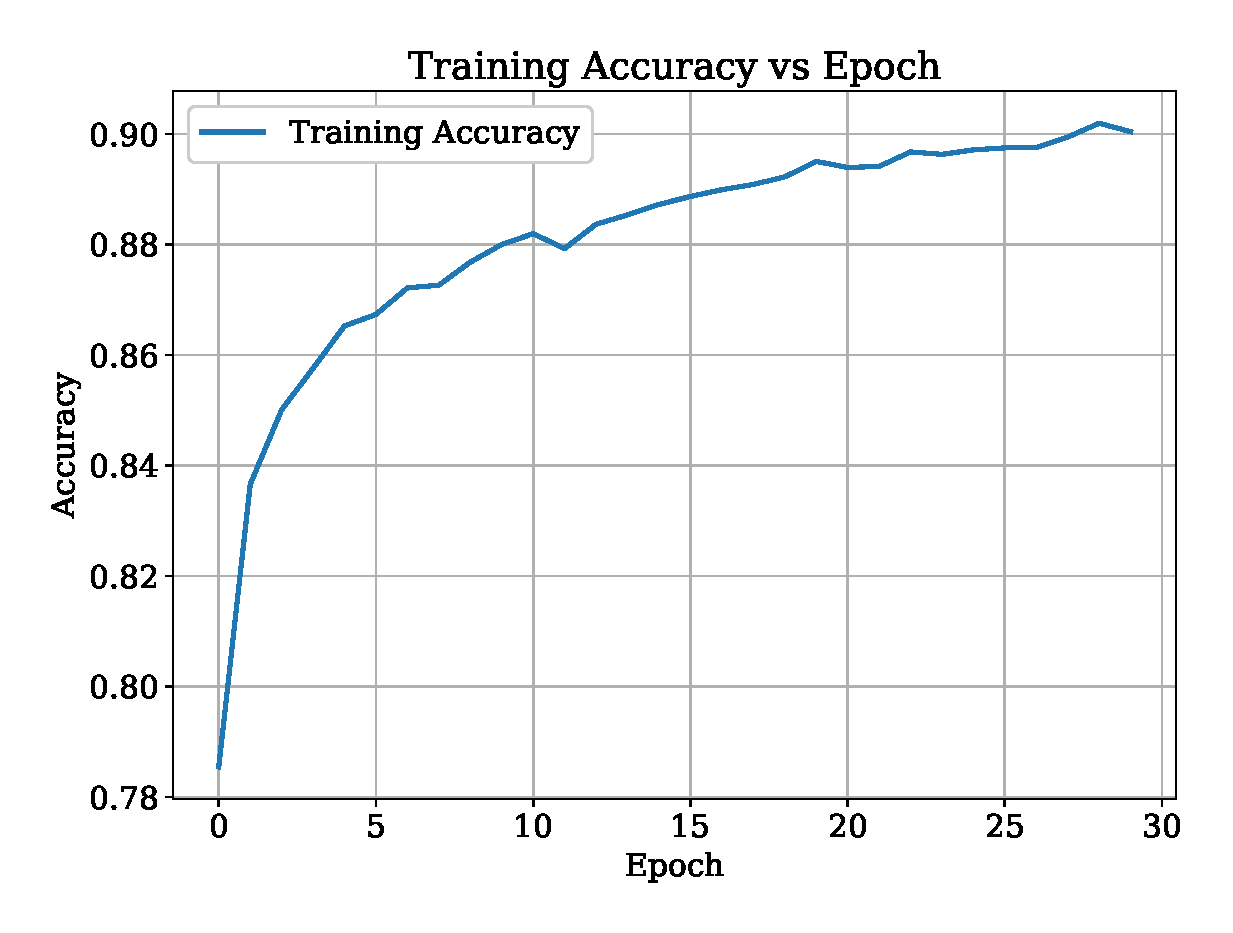
\includegraphics[width=0.75\linewidth]{Training_Accuracy.eps}
\caption{Training Accuracy versus Epoch}
\end{figure}

\textbf{Inference:}

The training accuracy increased steadily over successive epochs before converging. This indicates that the model had successfully learned meaningful feature representations from the training dataset.

\begin{figure}[H]
\centering
\includegraphics[width=0.75\linewidth]{Validation_Accuracy.eps}
\caption{Validation Accuracy versus Epoch}
\end{figure}

\textbf{Inference:}

The validation accuracy followed a trend similar to the training accuracy and stabilized after several epochs. The small gap between the training and validation curves indicates good generalization with limited overfitting.

\begin{figure}[H]
\centering
\includegraphics[width=0.75\linewidth]{Training_Loss.eps}
\caption{Training Loss versus Epoch}
\end{figure}

\textbf{Inference:}

The training loss decreased consistently throughout the learning process, indicating effective optimization of the model parameters and the convergence towards a lower error.

\begin{figure}[H]
\centering
\includegraphics[width=0.75\linewidth]{Validation_Loss.eps}
\caption{Validation Loss versus Epoch}
\end{figure}

\textbf{Inference:}

The validation loss has decreased rapidly during the initial epochs and later it stabilized. The absence of a significant increase in the validation loss suggests that the model had generalized well on unseen data.

\begin{figure}[H]
\centering
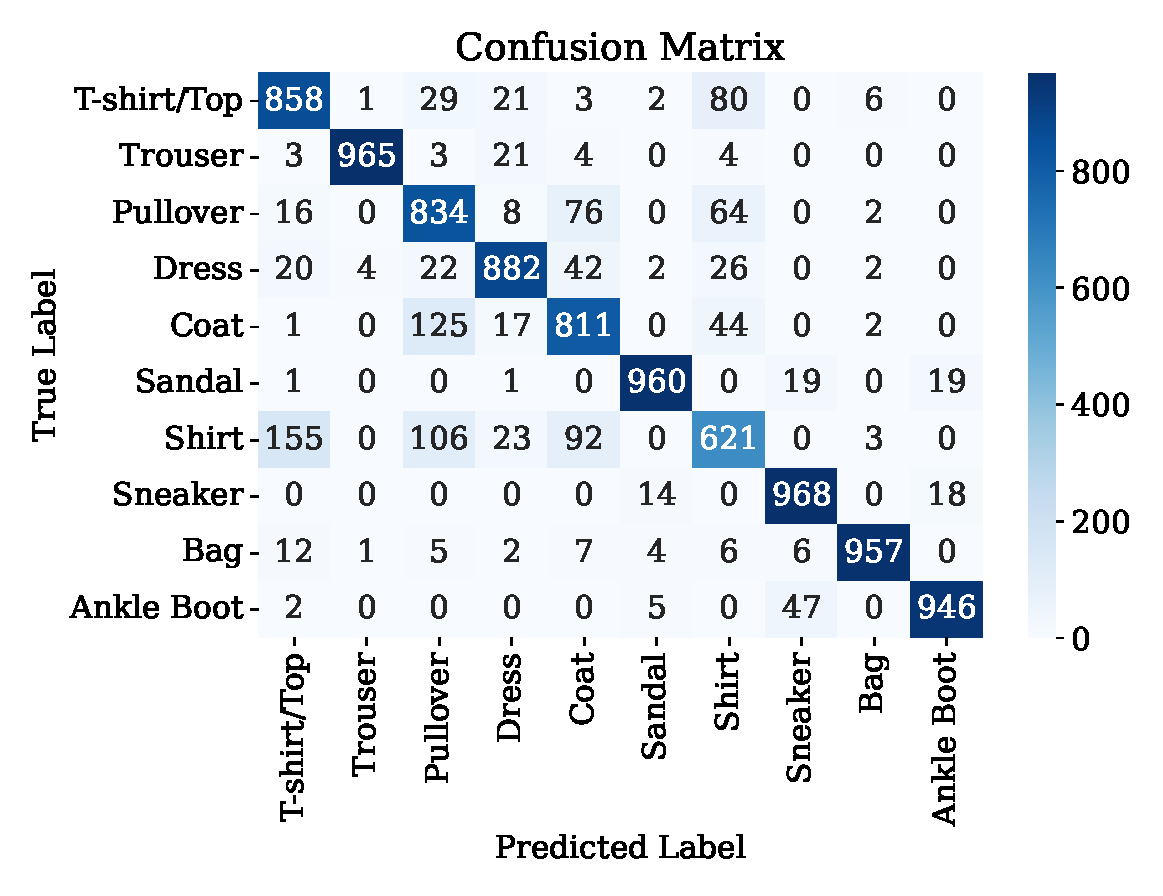
\includegraphics[width=0.85\linewidth]{Confusion_Matrix.eps}
\caption{Confusion Matrix of the Baseline MLP}
\end{figure}

\textbf{Inference:}

Most predictions lie along the main diagonal, indicating correct classification for the majority of test samples. Misclassifications primarily occur between visually similar categories such as Shirt, Pullover, and Coat, which share overlapping visual characteristics.

\begin{figure}[H]
\centering
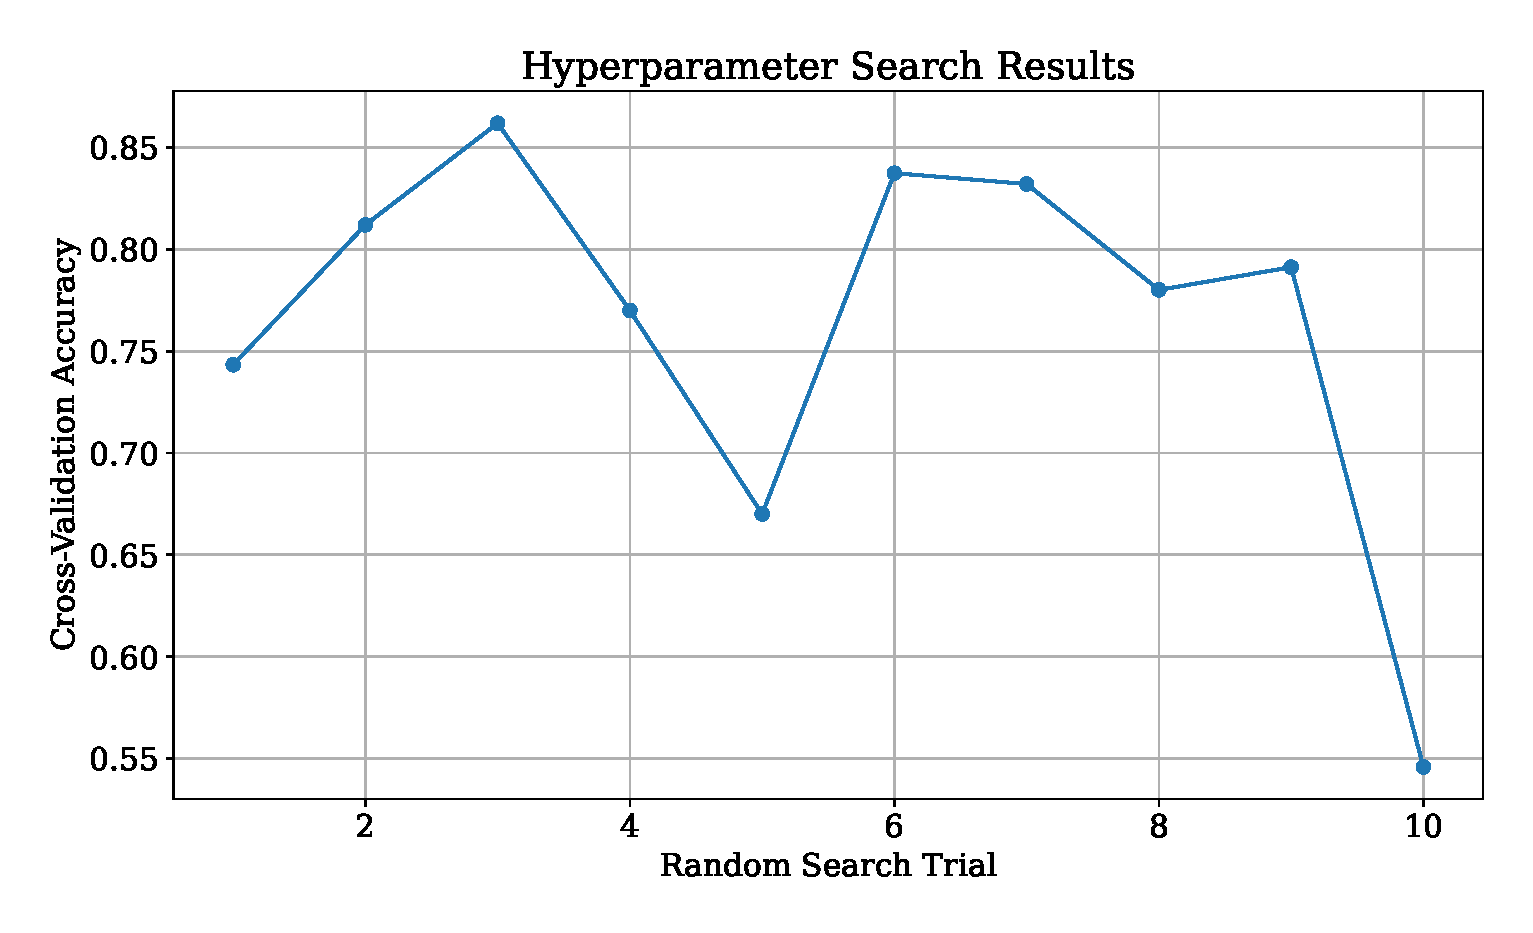
\includegraphics[width=0.75\linewidth]{Hyperparameter_Search.eps}
\caption{Hyperparameter Search Performance}
\end{figure}

\textbf{Inference:}

Different hyperparameter combinations produced varying cross-validation accuracies during Randomized Search. The search successfully identified a competitive configuration for retraining the optimized MLP model.

\begin{figure}[H]
\centering
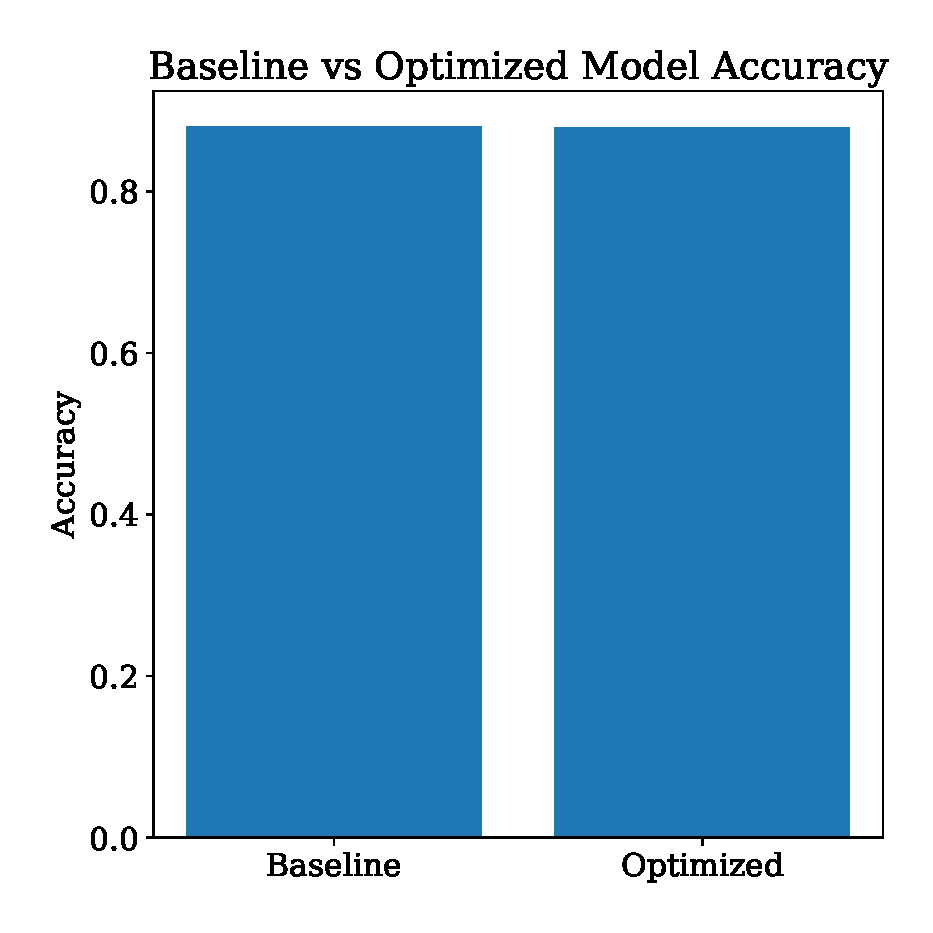
\includegraphics[width=0.65\linewidth]{Model_Comparison.eps}
\caption{Comparison of Baseline and Optimized MLP Accuracy}
\end{figure}

\textbf{Inference:}

The optimized model achieved performance comparable to the baseline model but did not exceed its testing accuracy. This indicates that the baseline architecture was already well suited for the Fashion-MNIST dataset, while the optimized configuration maintained similar generalization performance. A likely factor might be using the subset of 12,000 training samples to reduce computational time.

\section*{10. Results}

\textbf{Table 1. Hyperparameters}

\begin{center}
\begin{tabular}{|p{6cm}|p{5cm}|}
\hline
Hyperparameter & Best Value\\
\hline
Hidden Layers & 3\\
Hidden Neurons & 128\\
Learning Rate & 0.001\\
Batch Size &32\\
Optimizer & rmsprop\\
Activation Function & tanh\\
Epochs & 30\\
Dropout Rate & 0.2\\
Cross Validation Accuracy & 0.8619\\
Testing Accuracy & 0.8790\\
\hline
\end{tabular}
\end{center}
\vspace{3mm}

\textbf{Performance Comparison}
\begin{tabular}{|p{4cm}|c|c|}
\hline
Metric & Baseline & Optimized\\
\hline
Accuracy&0.880200&0.879000\\
Precision&0.881263&0.878630\\
Recall&0.880200&0.879000\\
F1-score&0.879768&0.877712\\
Training Time&2 min (approx)&30 min (approx)\\
\hline
\end{tabular}

\section*{11. Discussion}

\begin{enumerate}

\item \textbf{Which optimization method was used?}

RandomizedSearchCV together with the SciKeras wrapper was used to perform automated hyperparameter optimization. A 5-fold cross-validation strategy haad been adopted to evaluate the different combinations of the hyperparameters and to identify a suitable MLP configuration.

\vspace{3mm}

\item \textbf{Which hyperparameters were selected?}

The optimized model was obtained by tuning the number of hidden layers, number of hidden neurons, the learning rate, optimizer, activation function, dropout rate, batch size, and the number of training epochs. The final values selected by RandomizedSearchCV are presented in the Results section.

\vspace{3mm}

\item \textbf{Did optimization improve performance?}

The optimized model achieved performance comparable to the baseline model but did not outperform it on the testing dataset. A likely contributing factor is that the hyperparameter search was performed using a reduced subset of 12,000 training samples to reduce computational time. Consequently, the selected hyperparameters may not represent the optimal configuration for the complete Fashion-MNIST dataset. however, the optimized model demonstrated similar generalization performance to the baseline model.

\vspace{3mm}

\item \textbf{Which hyperparameter had the greatest impact?}

Among the tuned parameters, the learning rate and optimizer had the greatest influence on the model's convergence and overall classification performance. The network architecture, including the number of hidden layers and neurons, also affected the model's learning capacity and generalization.

\vspace{3mm}

\item \textbf{Compare Grid Search and Randomized Search.}

Grid Search evaluates every possible combination of hyperparameters, making it computationally expensive for large search spaces. In contrast, Randomized Search evaluates only a randomly selected subset of combinations, significantly reducing computation time while still identifying competitive hyperparameter configurations. Therefore, Randomized Search is more suitable for deep learning models with numerous tunable parameters.

\vspace{3mm}

\item \textbf{Recommend the best MLP configuration.}

For this experiment, the baseline MLP architecture consisting of two hidden layers with 128 and 64 neurons, ReLU activation, the Adam optimizer, categorical cross-entropy loss, and a batch size of 32 is recommended. Although Randomized Search produced a competitive model, the baseline configuration achieved marginally better testing accuracy while maintaining a simpler architecture.

\end{enumerate}

\section*{12. Conclusion}

In this experiment, a Multi-Layer Perceptron (MLP) was successfully implemented for multi-class image classification using the Fashion-MNIST dataset. The dataset was preprocessed by flattening the $28 \times 28$ grayscale images into 784-dimensional feature vectors, normalizing the pixel values to the range $[0,1]$, and converting the class labels into one-hot encoded vectors suitable for categorical classification. A baseline MLP architecture consisting of two hidden layers with ReLU activation and a Softmax output layer was developed using TensorFlow/Keras and trained using the Adam optimizer with categorical cross-entropy loss.

The trained model demonstrated strong classification performance on the Fashion-MNIST test dataset, achieving high accuracy, precision, recall, and F1-score. The confusion matrix indicated that the majority of test images were classified correctly, while a small number of misclassifications occurred between visually similar clothing categories such as shirts, pullovers, and coats. The training and validation accuracy and loss curves showed stable convergence, indicating that the network learned meaningful representations without significant overfitting.

Automated hyperparameter optimization was then performed using RandomizedSearchCV with the SciKeras wrapper to explore different combinations of hidden layers, hidden neurons, learning rates, optimizers, activation functions, dropout rates, batch sizes, and training epochs. Although the optimized model achieved performance comparable to the baseline model, it did not produce a higher testing accuracy. A likely reason is that the hyperparameter search was conducted on a reduced subset of 12,000 training samples to reduce computational time, which may have limited the ability of the search process to identify the globally optimal configuration for the complete dataset.

Overall, this experiment provided practical experience in the complete deep learning workflow, including data preprocessing, neural network design, model training, performance evaluation, and hyperparameter optimization. It also demonstrated that while automated hyperparameter optimization is a powerful technique for improving model performance, a well-designed baseline architecture can already achieve highly competitive results on balanced benchmark datasets such as Fashion-MNIST. The experiment highlights the importance of selecting appropriate network architectures, optimization strategies, and evaluation metrics when developing deep learning models for image classification tasks.


\section*{13. Report Contents}

Include Objective, Theory, Dataset, Experimental Procedure, Source Code, Hyperparameter Optimization, Results, Plots with Inference, Discussion, Conclusion and References.

\section*{14. References}
\begin{enumerate}
\item Goodfellow et al., \emph{Deep Learning}.
\item Bishop, \emph{Pattern Recognition and Machine Learning}.
\item Haykin, \emph{Neural Networks and Learning Machines}.
\item Fashion-MNIST Dataset.
\item TensorFlow/Keras Documentation.
\end{enumerate}

\section*{Aditional Exercise}
\section{Objective}

The objective of this experiment is to implement and analyze a Multi-Layer Perceptron (MLP) for solving the XOR classification problem. The experiment demonstrates the limitation of a single-layer perceptron on non-linearly separable data and illustrates how the introduction of a hidden layer enables successful learning. The model is implemented using TensorFlow and evaluated using training accuracy, loss, and prediction results.

\section{Experimental Procedure}

The experiment consists of two parts. In the first part, a single-layer perceptron is implemented from scratch to classify the XOR dataset. Since XOR is not linearly separable, the perceptron fails to converge even after multiple training epochs.

In the second part, a Multi-Layer Perceptron (MLP) is implemented using TensorFlow. The network consists of one hidden layer with eight neurons using the hyperbolic tangent (tanh) activation function and an output neuron with the sigmoid activation function. The model is trained using the Adam optimizer with a learning rate of 0.05 for 1000 epochs. The training process is analyzed using accuracy and loss curves, and the final predictions are evaluated.

\section{Network Architecture}

The architecture of the implemented Multi-Layer Perceptron is summarized in Table~\ref{tab:architecture}.

\begin{table}[H]
\centering
\caption{MLP Architecture}
\label{tab:architecture}
\begin{tabular}{|c|c|}
\hline
Input Layer & 2 Neurons \\ \hline
Hidden Layer & 8 Neurons (tanh) \\ \hline
Output Layer & 1 Neuron (sigmoid) \\ \hline
Optimizer & Adam \\ \hline
Learning Rate & 0.05 \\ \hline
Loss Function & Binary Crossentropy \\ \hline
Epochs & 1000 \\ \hline
\end{tabular}
\end{table}

\section{Results}

The single-layer perceptron was unable to classify the XOR dataset because the classes are not linearly separable. The training error did not converge to zero even after the maximum number of epochs.

The Multi-Layer Perceptron successfully learned the XOR function and achieved perfect classification of all four input combinations. The training accuracy approached 100\%, while the binary crossentropy loss decreased steadily during training.

\section{Results}

The single-layer perceptron was unable to classify the XOR dataset because the classes are not linearly separable. The training error did not converge to zero even after the maximum number of epochs.

The Multi-Layer Perceptron successfully learned the XOR function and achieved perfect classification of all four input combinations. The training accuracy approached 100\%, while the binary crossentropy loss decreased steadily during training.

\begin{figure}[H]
\centering
\includegraphics[width=0.65\textwidth]{XOR_Non_Convergence.eps}
\caption{Training error versus epoch for the single-layer perceptron on the XOR dataset.}
\label{fig:xor_non}
\end{figure}
\textbf{Inference:} The single-layer perceptron fails to solve the XOR problem because the classes are not linearly separable. The training error does not converge to zero even after multiple epochs.

\begin{figure}[H]
\centering
\includegraphics[width=0.65\textwidth]{Training_Accuracy_XOR.eps}
\caption{Training accuracy of the Multi-Layer Perceptron.}
\label{fig:accuracy}
\end{figure}
\textbf{Inference:} The training accuracy gradually increases and reaches 100\%, indicating that the Multi-Layer Perceptron successfully learns the XOR function.

\begin{figure}[H]
\centering
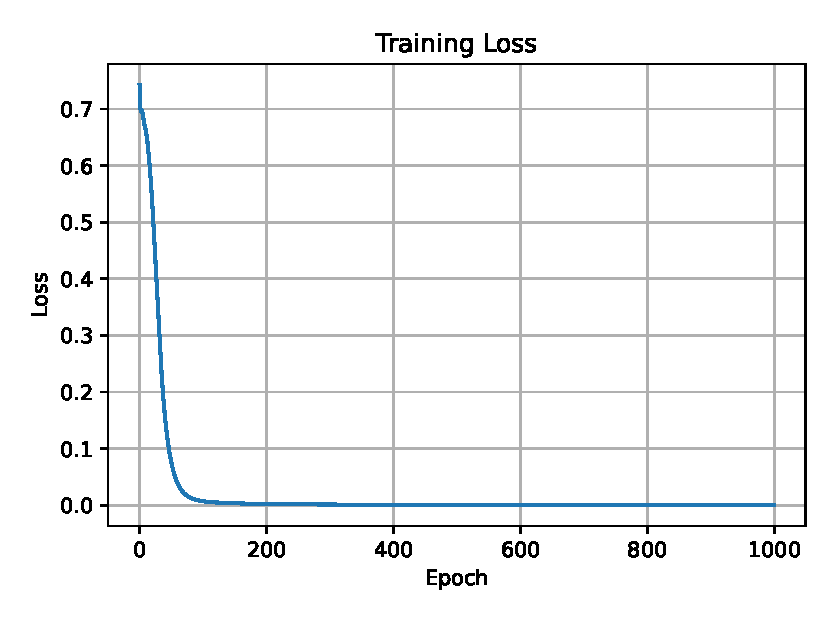
\includegraphics[width=0.65\textwidth]{Training_Loss_XOR.eps}
\caption{Training loss of the Multi-Layer Perceptron.}
\label{fig:loss}
\end{figure}
\textbf{Inference:} The binary crossentropy loss decreases steadily throughout training, demonstrating effective optimization and successful convergence of the neural network.

\begin{figure}[H]
\centering
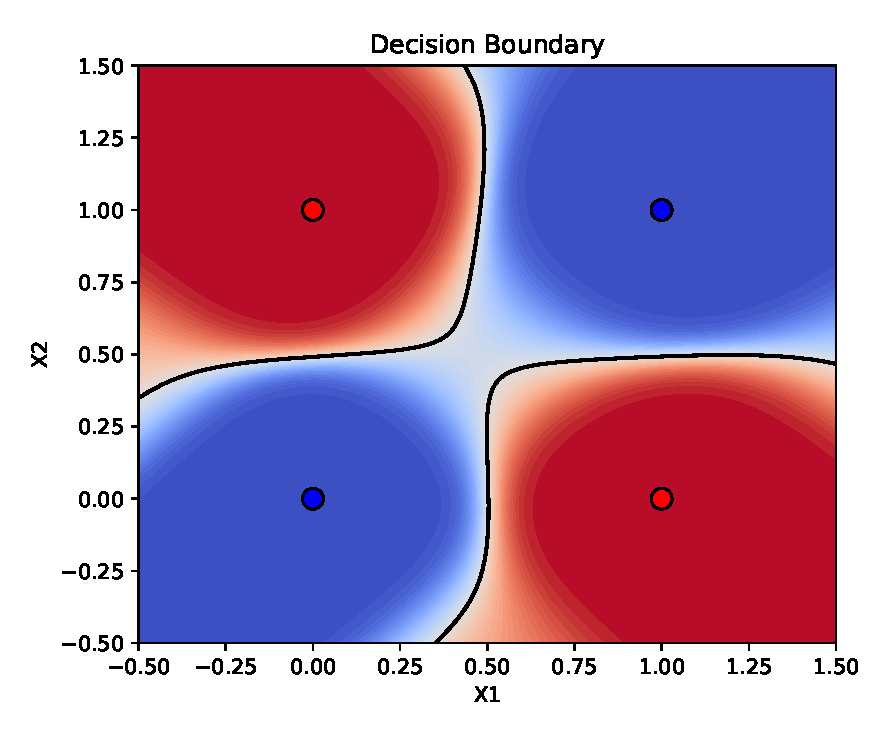
\includegraphics[width=0.65\textwidth]{Decision_Boundary.eps}
\caption{Decision boundary learned by the Multi-Layer Perceptron for the XOR problem.}
\label{fig:boundary}
\end{figure}



\section{Conclusion}

The experiment demonstrated the limitation of the single-layer perceptron on the XOR problem and highlighted the capability of the Multi-Layer Perceptron to solve non-linearly separable classification tasks. By introducing a hidden layer and nonlinear activation functions, the network successfully learned the XOR relationship and achieved perfect classification accuracy. The accuracy, loss, and decision boundary plots confirmed the convergence and effectiveness of the implemented neural network.

\end{document}
